This chapter is structured in the three main section, labeled \emph{SoA in Embedded System (Embedded SoA)}, \emph{Safety services} and \emph{Use Case: Error Detection Service}. 

The first section deals extensively with the possible application of the service oriented design paradigm in embedded system and deals with the challenges this approach has to face when approached with safety-critical requirements. Moreover, the differences to conventional SoAs, as Web application is investigated in detail. 
The second section presents xx services, which are relevant for \emph{functional safety} in detail and presents their intended functionality, as well as possible implementations in terms of an architecture.

The final part consists of a simplified use case, dealing with the design of an error detection service with respect to the design phases \emph{service investigation/planning}, \emph{service inventory analysis}, \emph{service oriented analysis} and \emph{service oriented design}.

Most of the findings and concepts in this chapter is ``not yet'' covered in literature, but is the result of numerous meetings and discussions.

\section{SoA in Embedded Systems (Embedded SoA)}
\subsection{Correlation of design philosophies}
\label{ch:correlation-of-design-philosophies}
The CBSE and SoA are coexisting design philosophies and usually either one or the other is applied in a given system. In contrast, Gleirscher and Vogelsang present in \cite{gleirscher2014} a proposal, how both paradigms can exist in parallel in a single system.

The presented system models consists of two layers with three different models. The \emph{feature layer} contains the \emph{feature hierarchy} model, which describes all the features a vehicle presents to its user. The \emph{platform layer}, in contrast, is the technical realization and consists of the \emph{service hierarchy} and the \emph{component model} \cite{gleirscher2014}.

This relation is depicted in figure \ref{fig:system-specification-models}.

\begin{description}
\item [Feature Hierarchy].
Alongside \emph{services} and \emph{components} their model disposes of a third hierarchy, denoted \emph{features}. 

According to \cite{gleirscher2014}, a feature ``is a behavioral property of a system observable (and influenceable) by its user.'' AUTOSAR describes it by the following quote:
\begin{quote}
\emph{``The term feature is commonly used in the software tool community to describe characteristics (functionality) of the software''} \cite{autosar_glossary}.
\end{quote}
The \emph{feature} has a many to many relationship to the services, since a service could offer various features, but one and the same feature, can also be offered by the very same service. For example the service \emph{braking service} could contain a \emph{safety braking mechanism}, which is responsible for performing an emergency brake when needed \cite{gleirscher2014}.

The set of features for a specific vehicle is given by its configuration in terms of hardware software, etc. A convertible car may include a feature for automatically opening and closing the top, while a sports car could allow to switch to a ``sport mode.''

\item [Service Hierarchy].
The services are the link between the features and the technical platform, they are realized on. A service can be provided either directly by a ``material component'', like a sensor or an actuator, or it can be composed out of various other services \cite{gleirscher2014}. For an acceleration sensor, the corresponding service would be the \emph{acceleration measurement}.

\item [Component Model].
The components are the material or immaterial, in other words hardware and software, parts of a system. Accordingly, a material part is for example a sensor and an immaterial part a communication software.
\end{description}

\begin{figure}[ht]
\centering
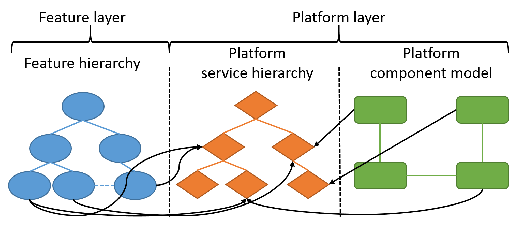
\includegraphics[scale=1.2]{system-specification-models.pdf}
\caption{Illustration of the overall system architecture by Gleirscher and Vogelsang \cite{gleirscher2014}.}
\label{fig:system-specification-models}
\end{figure}







\subsection{Difference between Web SoA and Embedded SoA}

The service oriented design paradigm was originally designed for the application in the web, which offered, more or less, ideal prerequisites for this kind of architectural style. There is an underlying network already available, which allows interconnection, and \emph{time constraints} are quite ..., because delays are unlikely to cause a disaster. Thus, it is not surprising that web services are the application area, where SoA has scored the highest market penetration \cite{rodrigues2011} \cite{buckl}.


In contrast to web services, \emph{embedded systems} are networks consisting of numerous interconnected nodes, with diverse measurement-, steering-, or computation capabilities. They have to face certain challenges like \emph{limited resources}, \emph{different complexity of hardware} \cite{scholz} \cite{sommer}. 

Some of the issues, the SoA has to face in embedded systems are described in the following.

\begin{description}
\item [Limited resources].
One obvious major drawback are the very limited resources in embedded systems, which are designed for highly specialized purposes and lack computation power as well as storage size \cite{rodrigues2011} \cite{scholz} \cite{sommer}.

Also the set of components is determined at assembly time ...

\item [Different levels of complexity].
The complexity usually varies greatly. The applied hardware components may include very simple sensors, with low resources and capabilities as well as very advanced nodes like MPSoCs) \cite{scholz} \cite{sommer}.

Accordingly, there are high level information systems services as well as low level, generic embedded system services. SoA has to deal with the connection and integration of them \cite{rodrigues2011}. Especially when it comes to the interaction of SoAs in embedded systems with SoAs at higher levels. 

\item [Event- and data-driven].
In contrast to web services, an embedded system disposes of (many) sensors which are interconnected in a network. Thus, the ad-hoc ``request-response message pattern'' which is known from web services does not work, for embedded systems are event- and data driven: For example a sensor measures some data and publishes it to all connected services. Those can then act according to the received input, e.g. trigger actuators or other services. This is denoted as ``fire and forget'' scheme \cite{sommer}.

\item [Lifespan of services].
Another difference to web services is the lifespan of services. While web services are used to work only a limited number of hours (or even minutes), the services in embedded systems could have application times of multiple years, e.g. a measurement service for a sensor \cite{buckl}.

\item [Dynamic character]. 
This is even aggravated by the dynamic character of embedded networks - \emph{``new nodes may enter the network, existing nodes may fail and network characteristics can change over time, especially if wireless communication media are used''} \cite{sommer}.

\item [Time constraints].
Embedded systems are time-critical, meaning that computation must be conducted within a given time window in order to allow the correct operation of the system. Especially in a safety-critical system like a vehicle, which is used to operate at high velocities, a violation of those time constraints could cause serious incidents.
\end{description}


These obstacles give reason to the statement that web services and safety-critical embedded systems are non-related areas \cite{rodrigues2011}.

Nevertheless, there are a lot of benefits in applying a service oriented architecture style, like decoupling configuration from environment, improvement of reuseability, maintainability, higher level of abstraction, interoperability, more interactive interfaces between devices and information systems.

% - Wiederverwertbarkeit - weniger entwicklungskosten
% - abstraktion von hardware -> dienst -> komponenten von verschiedenen herstellern
\cite{buckl}.
% - soa saves costs for hardware acquisition and infrastructure management \cite{sommer}

The SoA paradigm offers a promising possibility to overcome many of embedded systems related drawbacks and implementing some of the stated advantages \cite{buckl} \cite{sommer}. Thus, it is not surprising that there are various different projects dedicated to investigate the applicability of SoA for embedded systems. Those include SIRENA, SOCRATES, OASiS, MORE, RUNES and $\varepsilon$SOA. In the proceeding the $\varepsilon$SOA project by Scholz, Sommer et al. \cite{scholz} \cite{sommer} \cite{buckl} will be investigated in more detail.

\subsubsection*{eSoA}
The $\varepsilon$SOA project from Sommer, Gaponova and Buckl from the Department of Informatics at TU München, is an approach to master the obstacles which come with applying service oriented architectures in embedded systems.

However, the proposed architecture omits some functionality which is included in 
conventional SoAs, like the dynamic detection of services within the network. Moreover it features \emph{long term service composition} and uses external tools for the reconfiguration. However, a necessary requirement is the ability to update deployed services and migrate services to new hardware without a complete system interrupt \cite{sommer}.

\subsubsection*{Embedded SoA}
Unfortunately, there are not many sources covering the topic of SoA in embedded systems yet. Accordingly, the term \emph{embedded SoA} does not appear in literature, but has been defined during the EMC2 project, in order to refer to service oriented architectures in embedded systems. The relation of ``embedded SoA'' to ``conventional SoA'' has been defined as it can be seen in figure \ref{fig:soa-and-esoa}. According to these findings the \emph{embedded SoA} operates at a lower, very hardware oriented level, with a predefined and unchanging component architecture. 

The SoA is located ``above'' embedded SoA and connected by interfaces. With regard to the example of a vehicle, the embedded SoA operates on elements like a power train, various devices (sensors, actuators, ...) etc, while SoA level contains the vehicle as overall system, but also other vehicles, which can be referred to as the \emph{System of Systems}.


\begin{figure}[ht]
\centering
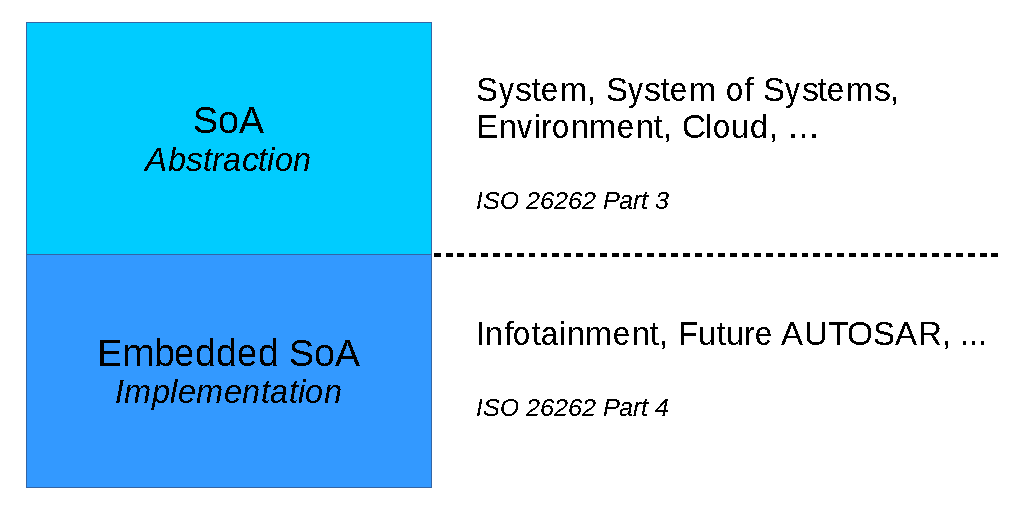
\includegraphics[scale=0.8]{soa-and-esoa.pdf}
\caption{Relation of service oriented architecture to service oriented architecture in embedded systems.}
\label{fig:soa-and-esoa}
\end{figure}









\subsection{SoA in automotive}

An important subpart of the EMC2 project is the investigation of the applicability of the SoA concepts for the automotive industry.

In the future of automotive all vehicles will be, most likely, interconnected with each other and also their environment. This could give them opportunities like automatically detecting whether the traffic lights are green at a crossing and acting automatically. Within this document those futuristic vehicles, which are interconnected with their environment, are referred to as ``connected cars''.




The opportunities and advantages of the SoA approach have been dealt with in the previous section. With respect to vehicles its major advantage would be the possibility to reduce the quantity of computation hardware, because at the present time each component disposes of his own dedicated hardware for this task. Many of those are unused for the majority of time, but nevertheless they come with a lot of extra weight. As stated in \cite[p.7]{marwedel}, ``Embedded systems should exploit the available hardware architecture as much as possible.''

The SoA approach might reduce not only the weight, but also the complexity and costs of the overall vehicle. So far it is usually the case that every vendor used its own proprietary network and additional hardware, prohibiting the application of hardware components from another vendor \cite{sommer}.

Despite of all these advantages, right now the SoA paradigm is hardly applicable for vehicles. On the one hand, this is due to the strict regulations which apply for safety critical real-time systems like vehicles, which do not yet include any requirements with respect to SoAs. In terms of automotive the safety aspect also has to be considered, since vehicles are safety-critical systems where an error or a malfunction can easily harm people \cite{kum}.

On the other hand, there are technical constraints. The AUTOSAR architecture, which is widely applied today, is not constructed for dynamic reconfiguration or binding of services, but everything has to be specified at building time. Still, there is already an approach by AUTOSAR, denoted ``Future AUTOSAR'', which is dealing with this very issue.

Although, the SoA for vehicles is still a long way ahead, it might be easier applicable at other levels, like the \emph{System of Systems} level, meaning other vehicles and the overall traffic. For self-driving vehicles there could be for example services for the communication with traffic lights. If the the traffic lights in Germany would use another service as the ones in Austria, a SoA would allow to dynamically bind the new service when the border is approached. There are already projects which are dealing with the communication at this level of implementation.


\subsubsection*{Location of the service repository}
The service repository is described in detail in section \ref{sef:soa-components}, but its exact location and implementation in connection with automotive remains ambigous.

For SoAs in automotive it is likely that there exist various distributed repositories. One repository inside of every vehicle, containing all the services provided by the vehicle itself, which is also accessible if the vehicle is operating in urban regions and is not able to connect to its environment. For the SoA inside the vehicle, there is no other possible location, because otherwise it would be operable only as long as it is connected to the Internet, or whatever platform, which is used for the interconnection with the environment.

For the scope of this document these repositories will be referred to by the term ``local service repository''. Examples for the services they hold are services which origin from hardware components of the vehicle like, acceleration measurement, temperature measurement, communication services and the like. But also safety critical services for fault- and error detection, which need to be available whenever the vehicle is operated.

The counterpart to the ``local service repository'' is denoted by ``external service repository''. This could also be physically distributed and holds mostly services which are needed for interacting with the environment. For ``self-driving''- or ``connected cars'' it could host all the services for managing the traffic. With an example: A traffic light in Graz publishes its service, ``Show me the traffic light signal'', somewhere on a server, where it is detected and bound by a vehicle driving in Graz, which is then able to decide whether it has to stop at an intersection.

Other services which could be located in this repository are \emph{update services}. If an update for an existing service in the local repository is available, the vehicle could detect this automatically and subsequently load and install the specific service.


\subsubsection*{Service Contract}

As already specified in section \ref{sec:soa-components}, the service contract is the complete and extensive description of the service and should contain, with regard to vehicles, Documents from AUTOSAR, the ISO 26262 standard and also documentation regarding \emph{functional safety}. It is more or less the goal of work package 1 of the EMC2 project to extend the \emph{service contract} by a functional safety part.

At the beginning of a service development process the contract is just an empty template which gets filled more and more as the development advances. A template, which could be used for the development of services in the automotive industry is already provided by the ARROWHEAD project.







\section{Safety services}

Disambiguation of Safety and security services 

\begin{figure}[ht]
\centering
\caption{Classification of various services into safety and security services.}
\label{fig:safety-and-security-services}
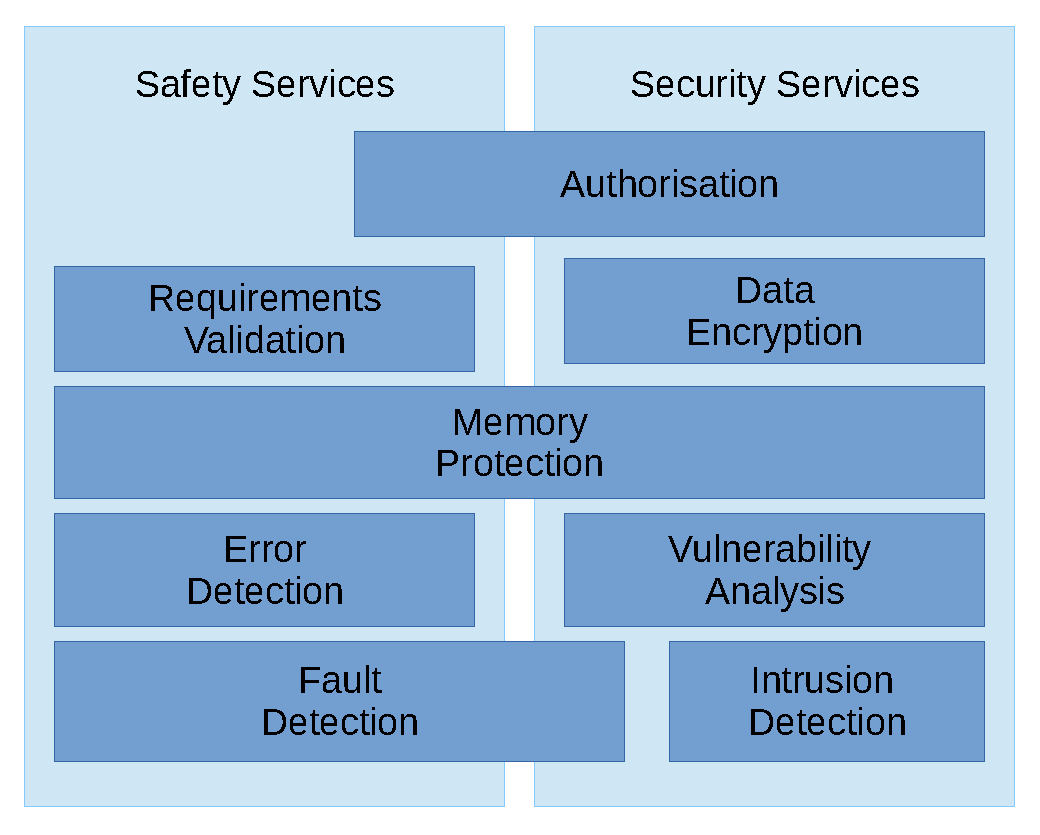
\includegraphics[scale=0.8]{safety-and-security-services.pdf}
\end{figure}

The most frequent application of service oriented architectures is in the field of Web services, where safety does not play a major role. However, in recent times this philosophy is also emerging in safety critical embedded systems, where specific safety and fault tolerance requirements have to be met.

There are many challenges for safety and security management in SoA systems, like the distributed hardware and software structure, loosely coupled components from different vendors, etc.


\subsection{Fault detection service (WDT)}

The fault detection service is described by means of its most prominent ``Vertreter'', the so called Watchdog Timer.

The \emph{Watchdog Timer (WDT)} is an fault detection service, which is, dependent from its implementation, also capable of detecting \emph{control flow errors}. Technically, the WDT is a simple timer circuit with a specified threshold time. If this limit is reached, it changes its state, which triggers further actions, like restarting a component or activating another safety service \cite{elattar2007}.

The advantages of the WDT is the simple design, which reduces the additional complexity of the overall system, as well as the costs. Concerning the functional principle, there are three slightly different designs, with individual capabilities and advantages \cite{elattar2007}.

\begin{description}
\item [Standard Watchdog Timer] .
With this basic setup, the service mirrored by the WDT periodically sends a simple heartbeat signal, indicating that the service is alive and active. This signal resets the timer. It a predefined amount of time elapsed, without an incoming signal, it is assumed that a fault has occurred and the WDT changes its state \cite{elattar2007}.

In terms of \emph{control flow errors} in a service, the execution sequence of the instructions of a service is changed, which means that the heartbeat signal may, or many not, be sent too late. Thus, in the latter case, the WDT is capable of detecting the error \cite{elattar2007}. 
The probability of noticing such an error is higher the closer the threshold time is to the time between the heartbeat signals.

\item [Windowed Watchdog Timer] .
The \emph{Windowed Watchdog Timer} is an improvement of the standard version, which is capable of detecting most of the \emph{control flow errors}. This is enabled by the application of two timers instead of one. With two timers the WDT is able to specify a time window, during which the heartbeat signal from the mirrored service must be received. The WDT is triggered if it receives a signal outside the window, or the timer reaches its threshold \cite{elattar2007}. This is illustrated in figure \ref{fig:windowed-watchdog-timer} with the $time$ on the x-axis and the Timers labeled $T1$ and $T2$.

In case of an \emph{control flow error} this signal is a bit ahead or past in time. The error detection coverage increases with narrowing the time window \cite{elattar2007}.  

The advantage of this design is clearly that it allows the detection of more errors, but on the other hand the implementation is slightly more complex.

\begin{figure}[ht]
\centering
\caption{Schematic design of a windowed watchdog timer \cite{elattar2007}.}
\label{fig:windowed-watchdog-timer}
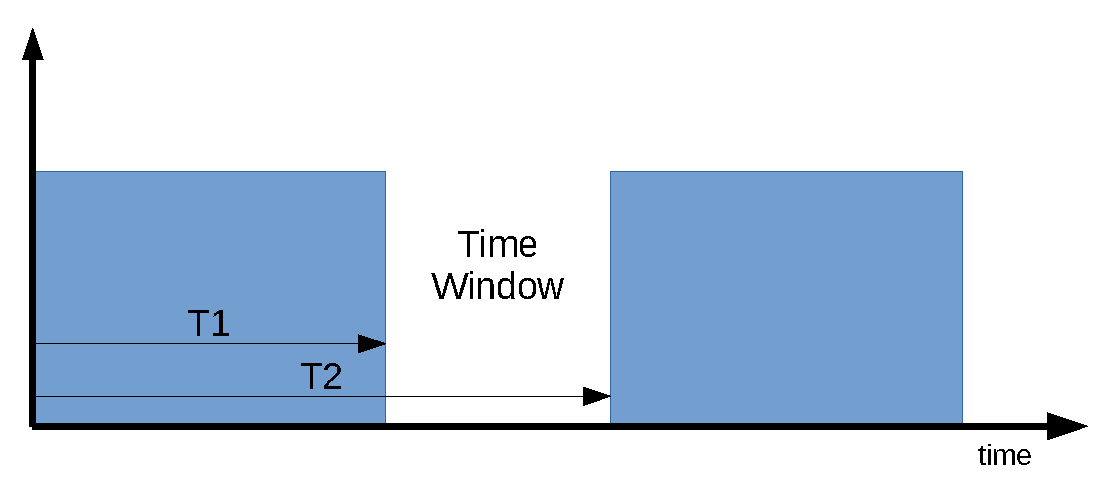
\includegraphics[scale=0.7]{windowed-watchdog-timer.pdf}
\end{figure}

\item [Sequenced Watchdog Timer] . 
This design is a further improvement of the \emph{Windowed Watchdog Timer} and bases on the same principle. In contrast, to the other designs, the signal sent from the mirrored service carries a sequenced parameter. Only if the signal arrives in time and within the specified time window, this parameter is evaluated and compared to a parameter inside the WDT. If those match the sequence variable in the WDT is incremented and the timer reseted, starting the cycle over again \cite{elattar2007}.
The whole proce ss is illustrated in figure \ref{fig:sequenced-watchdog-timer}.

The disadvantage of this design is the clearly higher complexity, for the \emph{Sequenced Watchdog Timer} must be capable of holding and modifying state information as well as comparing it to received information.

\begin{figure}[ht]
\centering
\caption{Schematic illustration of the working process of a \emph{Sequenced Watchdog Timer} \cite{elattar2007}.}
\label{fig:sequenced-watchdog-timer}
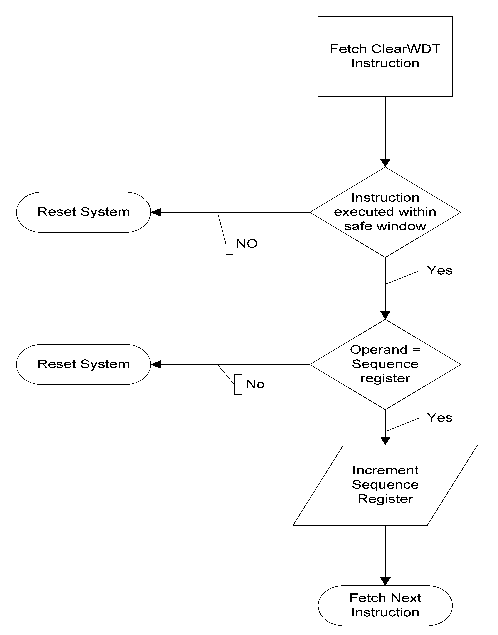
\includegraphics[scale=1.0]{sequenced-watchdog-timer.pdf}
\end{figure}

\end{description}

\begin{figure}[ht]
\centering
\caption{Example architecture for an \emph{fault detection service}, like a WDT.}
\label{fig:fault-detection-service}
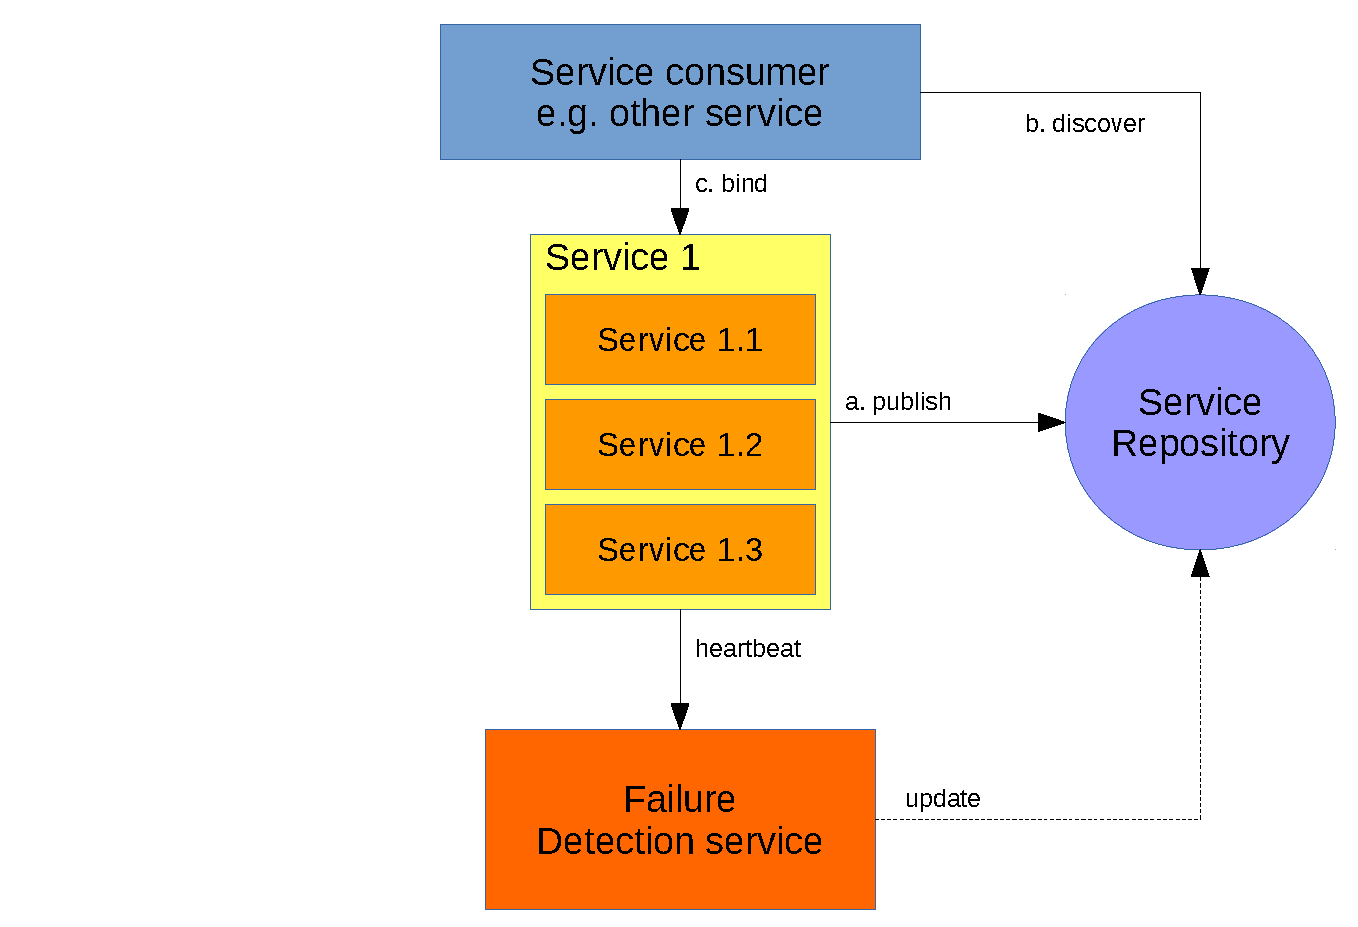
\includegraphics[width=\textwidth]{fault-detection-service.pdf}
\end{figure}



\subsection{Error detection service}

\begin{figure}[ht]
\centering
\caption{Example architecture for an \emph{error detection service}.}
\label{fig:error-detection-service}
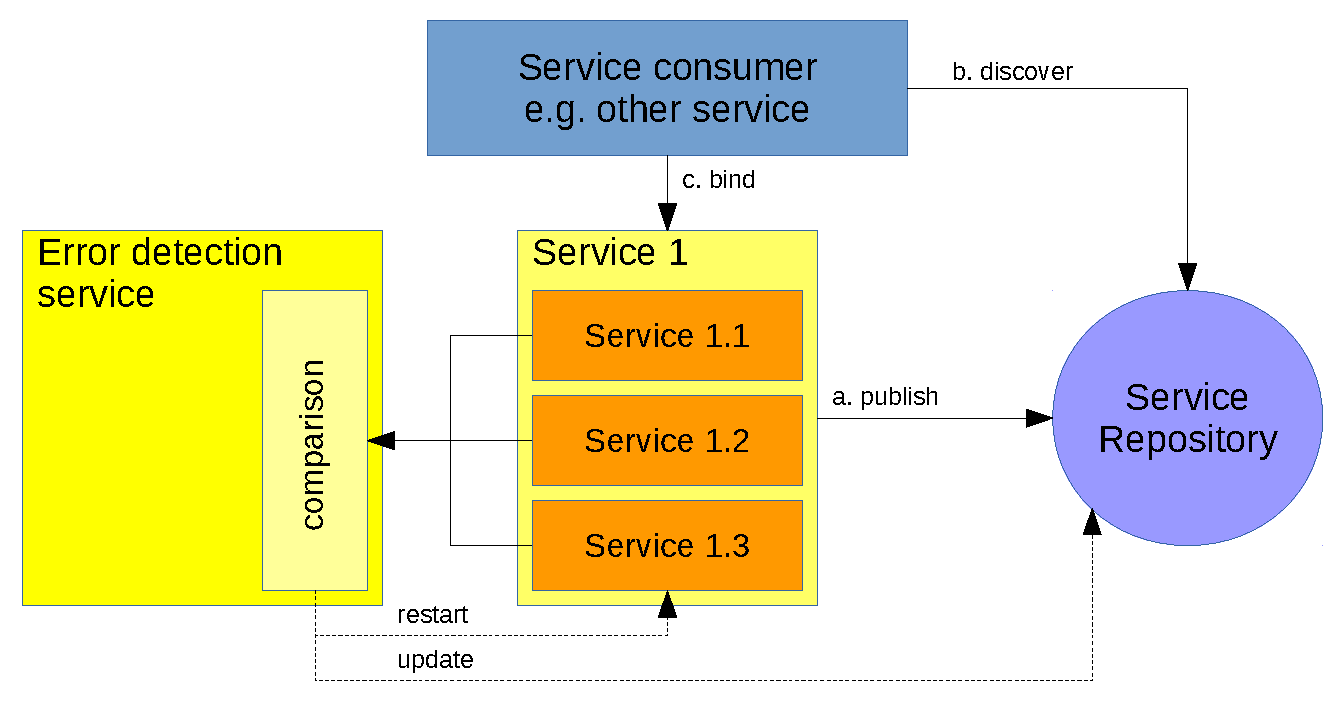
\includegraphics[width=\textwidth]{error-detection-service.pdf}
\end{figure}


\subsection{Memory Protection Service}

\emph{Memory protection} is related to \emph{safety} as well as \emph{security}. It is a method for preventing processes or users from accessing memory that is not allocated to them.

Former embedded systems, or such that are small in size, do not necessarily require memory protection mechanisms, but modern, large scale system, have several advantages ... and with the increase of computing power the overhead is no longer crucial \cite{yamada2008}.

There are several aspects that stress the need for memory protection in embedded systems:
\begin{itemize}
\item It can serve as fault and error detection and containment mechanism, preventing a failure of one service to propagate and infecting the whole system \cite{yamada2008}.
\item It is an important aid in the development process and helps at debugging by identifying ``illegal'' behaviour of erroneous services \cite{yamada2008}.
\item It is also crucial from a security point of view, because it prohibits unauthorised access.
\end{itemize}

It is bizarre that memory protection is nowhere mentioned in connection with service oriented architectures 

% + connection to the outside world 

\subsection{Orchestration Management Service}

\section{Use Case: Error Detection Service}
\subsection{Service Investigation/Planning}
\subsection{Service inventory analysis}
\subsection{Service oriented analysis}
\subsection{Service oriented design}